\documentclass[mathserif, aspectratio=169]{beamer}
\usetheme{odenpecos}
\setbeamertemplate{itemize/enumerate body begin}{\fontsize{8.8}{9}\selectfont}
\setbeamertemplate{itemize/enumerate subbody begin}{\fontsize{7.5}{8}\selectfont}
\setbeamertemplate{itemize/enumerate subsubbody begin}{\fontsize{7.5}{8}\selectfont}

% default search path for figures
\graphicspath{{./shared_figures/}{./figures/}}

\newcommand{\zapspace}{\topsep=0pt\partopsep=0pt\itemsep=0pt\parskip=0pt}

\usepackage{multicol}
\usepackage{pict2e}
\usepackage{esdiff}
\usepackage{multimedia}
\usepackage{verbatim}
\usepackage{mhchem}

\usepackage[percent]{overpic}
\usepackage[absolute,overlay]{textpos}

\newcommand{\overbar}[1]{\mkern 1.5mu\overline{\mkern-1.5mu#1\mkern-1.5mu}\mkern 1.5mu}
\newcommand{\pp}[2]{\frac{\partial #1}{\partial #2}}
\newcommand{\dd}[2]{\frac{d #1}{d #2}}
\newcommand{\DD}[2]{\frac{D #1}{D #2}}
\newcommand{\mm}{\mathbf{minmod}}
\def\etal{{\it et al~}}
\newcommand{\be}{\begin{eqnarray}}
\newcommand{\ee}{\end{eqnarray}}
\newcommand{\mbb}[1]{\mathbb{#1}} % math blackboard bold
\newcommand{\mcal}[1]{\mathcal{#1}} % math blackboard bold
\newcommand{\mbf}[1]{\mathbf{#1}} % math bold face (for vectors)
\newcommand{\sbf}[1]{\boldsymbol{#1}} % bold face for symbols
\newcommand{\jump}[1]{\llbracket #1 \rrbracket} % jump operator
\newcommand{\avg}[1]{\langle #1 \rangle} % average operator
\newcommand{\rarrow}{\rightarrow}
\newcommand{\Rarrow}{\Rightarrow}
\newcommand{\LRarrow}{\Leftrightarrow}
\newcommand{\vvvert}{|\kern-1pt|\kern-1pt|}
\newcommand{\enorm}[1]{\vvvert #1 \vvvert}
\newcommand{\nutil}{\tilde{\nu}}
\newcommand{\Var}{\mathrm{Var}}
\newcommand{\Cov}{\mathrm{Cov}}


\definecolor{MyDarkGreen}{rgb}{0,0.45,0.08}
\newcommand{\myred}[1]{{\color{red} #1}}
\newcommand{\myblue}[1]{{\color{blue} #1}}
\newcommand{\mygreen}[1]{{\color{MyDarkGreen} #1}}

\newcommand{\sa}{\nu_{\mathrm{sa}}}
\newcommand{\tep}{\tilde{\epsilon}}
\newcommand{\Ssd}{\mathcal{S}} % source term due to slow derivative
\newcommand{\ud}{\,\mathrm{d}}

\newcommand{\Mach}[1]{\ensuremath{\mbox{Ma}_{#1}}}
\newcommand{\Reynolds}{\ensuremath{\mathit{Re}}}
\newcommand{\DensityRat}{\ensuremath{\mathit{DR}}}
\newcommand{\BlowRat}{\ensuremath{\mbox{BR}}}
\newcommand{\VelRat}{\ensuremath{\mathit{VR}}}
\newcommand{\Tau}{\ensuremath{\mathrm{T}}}

\newcommand{\wall}     {\ensuremath{\mathrm{w}}}   % wall subindex
\newcommand{\awall}    {\ensuremath{\mathrm{aw}}}  % adiabatic wall subindex

\newcommand{\commentout}[1]{}

\newcommand{\vect}[1]{\boldsymbol{#1}}
\usepackage{mleftright}
\newcommand{\of}[1]{\mleft( #1 \mright)}
\newcommand{\vth}{v_{\textrm{th}}}
\newcommand{\reals}{\mathbb{R}}
\newcommand{\myint}{\int\limits}
\newcommand{\ddt}[1]{\partial_t #1}
\newcommand{\RR}{\mathbb{R}}
\newcommand{\vr}{v}
%\newcommand{\vtheta}{\theta_{\vect{v}}}
%\newcommand{\vphi}{\varphi_{\vect{v}}}
%\newcommand{\vr}{v_{r}}
\newcommand{\vtheta}{v_{\theta}}
\newcommand{\vphi}{v_{\varphi}}
\newcommand{\vomega}{v_{\omega}}
\newcommand{\vrunit}{\hat{\vect{v}}_{r}}
\newcommand{\vthetaunit}{\hat{\vect{v}}_{\theta}}
\newcommand{\vphiunit}{\hat{\vect{v}}_{\varphi}}
\DeclareMathOperator{\variance}{Var}

\begin{document}
% disable nav
\setbeamertemplate{navigation symbols}{}

% ---------------------------------------------------------------
% Oden/Pecos title page

%\hoffset=.16in
%
%\begin{frame}[plain,t]{}
%\makeatletter
%%\vspace*{0.85cm}
%%\vspace*{0.65cm}
%\includegraphics[height=0.9in,trim=50 40 40 0, clip]{PMSc_159_university_formal_horizontal.pdf} \newline
%%\vspace*{0.3cm}
%\begin{columns}[T,onlytextwidth]
%\column{.8\textwidth}
%{\bf \color{burntorange} \fontfamily{bch}\selectfont 
%% -- Set talk title here
%Solving the Boltzmann equation for electron kinetics using Petrov-Galerkin approach
%% --
%}
%\end{columns}
%\vspace*{.15cm}
%\rule{.8\textwidth}{0.6pt} \newline
%
%\vspace*{0.05cm}
%\setstretch{0.65}
%{\fontfamily{phv}\selectfont
%  { \scriptsize
%    % -- define presenter, authors here
%    Milinda Fernando, Daniil Bochkov, Todd Oliver, George Biros\newline
%    % --
%  }
%  {\color{burntorange} \tiny
%    % -- define role, meeting event, location, etc
%    Year-1 Review $\cdot$ August, 2021 $\cdot$ Austin, TX
%    % --
%  }
%}
%
%\vspace*{1cm}
%%\includegraphics[height=0.3in]{figures/pecos_orange1.png}
%\begin{columns}
%\begin{column}{0.8\linewidth}
%\includegraphics[height=0.5in]{oden_pecos_2020_wordmark.png}\\
%{\scriptsize \url{https://pecos.oden.utexas.edu}}
%\end{column}
%
%\begin{column}{0.2\linewidth}
%\includegraphics[height=0.6in]{psaap3-logo.png}
%\end{column}
%\end{columns}
%
%\end{frame}
%\hoffset=0in
% -- end title slide ---------------------------------------------


%\begin{frame}
%	\frametitle{}
%	\begin{itemize}
%		\item Mass matrix for splines is ill-conditioned. 
%		\item Using Cholesky factorization based inversion has improved the projection coefficient accuracy for b-splines. 
%	\end{itemize}
%\begin{table}
%	\centering
%	\begin{tabular}{cc}
%		svd pseudo-inverse $\sigma_{c} = 10^{-15}\max\sigma$ &  Cholesky factored inverse \\
%		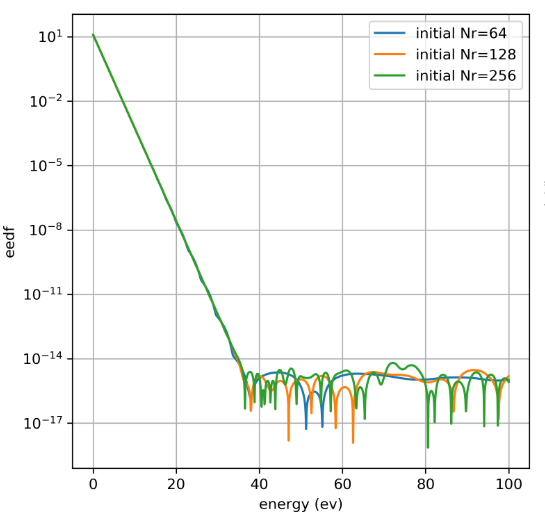
\includegraphics[width=0.35\textwidth]{figures/svd_pseudo_inv.png} &
%		\includegraphics[width=0.35\textwidth]{figures/cholesky_inv.png} 
%	\end{tabular}
%\end{table}
%\end{frame}

\begin{frame}
\begin{itemize}
\item A general ionization collision (infinitely heavy atoms):
\begin{align*}
\vect{p}_e \rightarrow \vect{p}_1 + \vect{p}_2
\end{align*}
\item Weak form:
\begin{multline*}
\left< C_i, \psi \right> 
= 
n_0
\int_{R^3 \cap u_e > \Delta E_i} d^3 \vect{p}_e
\int_{0}^{u_{e} - \Delta E_i} d u_1 
\int_{S^2} d\Omega\of{\hat{\vect{p}}_1}
\int_{S^2} d\Omega\of{\hat{\vect{p}}_2}
\frac{ p_{e} }{ m }
\sigma_{i} \of{ \vect{p}_{e} \rightarrow u_{1}, \hat{\vect{p}}_{1}, \hat{\vect{p}}_{2}}
\\
\times
f_e\of{\vect{p}_e} \left( 2 \psi\of{\vect{p}_1^{post}}  
- \psi\of{\vect{p}_e} \right)
\end{multline*}
where
\begin{align*}
u_e &= \frac{p_e^2}{2m}
\\
\vect{p}_1^{post} &= \hat{\vect{p}}_1 \sqrt{2 m u_1}
\end{align*}
\end{itemize}

\end{frame}



\begin{frame}
\begin{itemize}
\item Case of equal energy splitting and uniform probability with respect to all angles
\begin{align*}
\sigma_{i} \of{ \vect{p}_{e} \rightarrow u_{1}, \hat{\vect{p}}_{1}, \hat{\vect{p}}_{2}}
=
\frac{\sigma_{i,tot} \of{ \vect{p}_{e} }}{(4\pi)^2} \delta\of{u_1 - \frac12 \left( u_{e} - \Delta E_i \right)}
\end{align*}
\item Can integrate out over $u_1$ and $\Omega\of{\hat{\vect{p}}_2}$:
\begin{align*}
\left< C_i, \psi \right> 
= 
n_0
\int_{R^3 \cap u_e > \Delta E_i} d^3 \vect{p}_e
\int_{S^2} d\Omega\of{\hat{\vect{p}}_1}
\frac{ p_{e} }{ m }
\frac{\sigma_{i,tot} \of{ \vect{p}_{e} }}{4\pi}
f_e\of{\vect{p}_e} \left( 2\psi\of{\vect{p}_1^{post}}  
- \psi\of{\vect{p}_e} \right)
\end{align*}
where now
\begin{align*}
\vect{p}_1^{post} &= \hat{\vect{p}}_1 \sqrt{m \left( u_{e} - \Delta E_i \right)}
\end{align*}

\item Note: potentially could be further reduced by noticing
\begin{align*}
\int_{S^2} d\Omega\of{\hat{\vect{p}}_1} \psi\of{\vect{p}_1^{post}} =
\int_{S^2} d\Omega\of{\hat{\vect{p}}_1} P_{kl} \of{p_1^{post}} Y_{lm}\of{\hat{\vect{p}}_1} 
\sim \delta_{0,l} P_{kl} \of{p_1^{post}}
\end{align*}

\end{itemize}
\end{frame}




%===============================================================================
\end{document}

